\documentclass[12pt]{article}
\usepackage{amsfonts,amssymb}
\usepackage{exercise}
\usepackage{amsmath}
\usepackage{amsthm}
\usepackage{hyperref}
\usepackage{graphicx}
\usepackage{listings}
%\documentstyle[12pt,amsfonts]{article}
%\documentstyle{article}

\setlength{\topmargin}{-.5in}
\setlength{\oddsidemargin}{0 in}
\setlength{\evensidemargin}{0 in}
\setlength{\textwidth}{6.5truein}
\setlength{\textheight}{8.5truein}
%
%\input ../adgeomcs/lamacb.tex
%\input ../mac.tex
%\input ../mathmac.tex
%
\input xy
\xyoption{all}
\def\fseq#1#2{(#1_{#2})_{#2\geq 1}}
\def\fsseq#1#2#3{(#1_{#3(#2)})_{#2\geq 1}}
\def\qleq{\sqsubseteq}
\newtheorem{theorem}{Theorem}
%cis51109hw1

%
\begin{document}
\begin{center}
\fbox{{\Large\bf Recursion}}\\
\vspace{1cm}
\end{center}

\vspace{0.5cm}\noindent

All code in this section will be in Python since that was the language of instruction in CIT591 (or 590). Even if you do not know Python, the syntax is easy enough to understand. You will not be asked to code in exams. A choice of language is just needed so that it is completely unambiguous as to what my program is doing.

\section*{Recursion}
The idea behind recursion is the same as that being used in proofs by induction. Can we show the fact that if a problem is solved (if a theorem is true) for smaller instances (for n-1, n-2 etc) then the problem is solvable (then the theorem is true) for the current instance (for n).

The canonical example used to introduce recursion in most CS classes is factorial. Factorial has this nice property that $factorial(n) = n \times factorial(n-1)$. So when you write the function recursively as follows

\begin{verbatim}
def factorial(n):
    if n == 0: return 1
    return n * factorial(n-1)
\end{verbatim}

there is level of trust that goes on that should not make you really question something along the lines of 'why should I believe factorial(n-1) will get computed correctly'. The correct way of thinking is to say let me assume factorial(n-1) is computed correctly. Can I do something with that?

\subsection*{Proving a program works!}

While no one really truly does this in the industry, it is important to know if a program really works. And by this we do not mean, is there a syntax error or a logical flaw. We are asking the question that in a world where the idea that you have (CS calls those algorithms) gets perfectly translated into code (in some non crazy programming language), can you prove that your program will work regardless of the input provided to it.

Now the current best practice in the industry to do this proof is to write a bunch of unit tests. But does unit testing equate to a proof of correctness?

Unfortunately, math will just laugh at that notion. Unit testing just amounts to proof by example. Wouldn't it be better if you could say it works for everything. That turns out to be a universal statement.

\medskip

So for factorial this is what you want to prove

This program will compute factorial correctly regardless of input! 

How do you actually write a proof? You rely on the fact that induction is recursion!

Here's a sketch of the proof.

Base case - observe that when n=0 then the program returns 1 and that happens to be the same as 0!

Induction hypothesis - we assume that factorial works just fine for 0,1,2,...,n-1

Now for computing factorial of $n$, see that the program computes it as $n \times factorial(n-1)$. But we know by induction that we actually have $factorial(n-1) = (n-1)!$.

So the program is just computing $n \times (n-1)!$. But that is just $n!$.

\section*{How long does it take?}

As noted before, in most cases in the industry, you do not care about proving the correctness of your code (depends on the industry of course). But you do care about how much time your program is going to take!

While there are several ways of measuring time, the theoretical computer science methodology is to basically focus on the particular aspect of scalability. 

Let us see this using a specific example. The simple problem of searching through an array.

\subsection*{Searching}

Consider the problem of searching for the number 97 in an array of integers. You would expect (and rightly so!) to spend less time searching for this number in an array of size 100 versus an array of size 1 million. 

Clearly the time taken in a search problem is dependent on the size of the array. But does it grow quadratically, exponentially, logarithmically etc. That is one of the big questions that this topic of analysis of algorithms would like to address.

\section*{Big-Oh}

The way a CS person expresses the time taken for an algorithm is to say the algorithm is O(f(n)). For instance the search problem above can easily be shown to be $O(n)$ (once you know the definition of O). So you will say 

Searching in an unsorted array is an Oh of n operation. 

or 

Searching is a linear operation.

Definition of big-oh: - 

Let f and g be two functions defined on some subset of the real numbers. One writes
\begin{align*}
f(x)=O(g(x))\text{ as }x\to\infty\,
\end{align*}

if and only if there is a positive constant $C$ such that for all sufficiently large values of $x$, $f(x)$ is at most $C$ multiplied by the absolute value of $g(x)$. That is, $f(x) = O(g(x))$ if and only if there exists a positive real number $C$ and a real number $n_0$ such that

\begin{align*}
|f(x)| \le \; C |g(x)|\text{ for all }x \ge n_0.
\end{align*}

While the formal definition is needed for the math's sake, most CS people think of it in terms of this graph

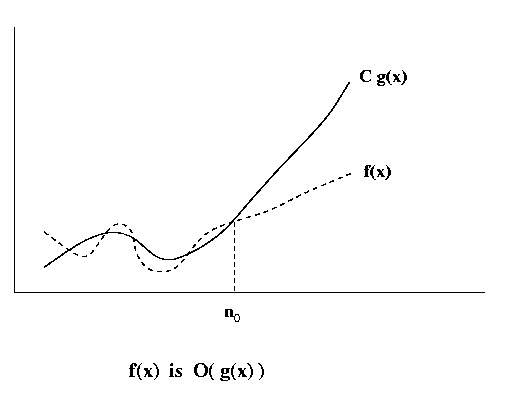
\includegraphics[scale=0.5]{bigO.png}

Beyond a certain point, a constant multiple of one of the functions dominates the other.

\medskip

\textbf{Example}

Show that $n^2 + 100n$ is $O(n^2)$.

\medskip

Show in class why in this case you can set $C$ to be a number like 200 and $x_0$ to be $2$. Obviously other values are possible but the thing about the $O$ analysis is that you can be sloppy


\subsection*{Sloppiness is ok?}

Algorithmic complexity is interesting in that it deals with inequalities more than equalities. So you will often look at the expression for time taken and draw conclusions very quickly by dropping terms. For instance if you compute the relationship between search time and the size of the array and say that it is $100n$, that is actually generally expressed as $0(n)$. 

The constants do matter, but first it is important to make an efficient algorithm in the big - O sense. If you have two competing algorithms that are both linear, then you can worry about the constants. But if you have one which is linear and one which is quadratic, it should be clear which one is to be picked.

Therefore, remember that you are allowed to do some sloppy math when you are analyzing algorithms. The key is to begin the sloppiness only after you have written a correct expression down and done some level of evaluation.


\section*{Mergesort}

Here is one version of the mergesort code in Python. 

\begin{verbatim}
def mergeSort(a):
    if len(a)==0 or len(a) == 1:
        return a
    else:
        firstHalf = mergeSort(a[:len(a)/2])
        secondHalf = mergeSort(a[len(a)/2:])
        return merge(firstHalf, secondHalf)

def merge(a1, a2):
    a3 = []
    len1 = len(a1)
    len2 = len(a2)
    i=j=0
    while i < len1 and j < len2:
        if a1[i] < a2[j]:
            a3.append(a1[i])
            i += 1
        else:
            a3.append(a2[j])
            j += 1
    # we would either have gone through
    # all of a1 or all of a2 by this time
    # just tack on the remainging stuff at the end
    if i < len1:
        a3.extend(a1[i:])
    if j < len2:
        a3.extend(a2[j:])
    return a3
\end{verbatim}


\end{document}



